\let\negmedspace\undefined
\let\negthickspace\undefined
\documentclass[journal]{IEEEtran}
\usepackage[a5paper, margin=10mm, onecolumn]{geometry}
%\usepackage{lmodern} % Ensure lmodern is loaded for pdflatex
\usepackage{tfrupee} % Include tfrupee package

\setlength{\headheight}{1cm} % Set the height of the header box
\setlength{\headsep}{0mm}     % Set the distance between the header box and the top of the text

\usepackage{gvv-book}
\usepackage{gvv}
\usepackage{cite}
\usepackage{amsmath,amssymb,amsfonts,amsthm}
\usepackage{algorithmic}
\usepackage{graphicx}
\usepackage{textcomp}
\usepackage{xcolor}
\usepackage{txfonts}
\usepackage{listings}
\usepackage{enumitem}
\usepackage{mathtools}
\usepackage{gensymb}
\usepackage{comment}
\usepackage[breaklinks=true]{hyperref}
\usepackage{tkz-euclide} 
\usepackage{listings}
% \usepackage{gvv}                                        
\def\inputGnumericTable{}                                 
\usepackage[latin1]{inputenc}                                
\usepackage{color}                                            
\usepackage{array}                                            
\usepackage{longtable}                                       
\usepackage{calc}                                             
\usepackage{multirow}                                         
\usepackage{hhline}                                           
\usepackage{ifthen}                                           
\usepackage{lscape}
\usepackage{multicol}
\begin{document}

\bibliographystyle{IEEEtran}
\vspace{3cm}

\title{12.130}
\author{EE25BTECH11012-BEERAM MADHURI}
% \maketitle
% \newpage
% \bigskip
{\let\newpage\relax\maketitle}

\renewcommand{\thefigure}{\theenumi}
\renewcommand{\thetable}{\theenumi}
\setlength{\intextsep}{10pt} % Space between text and floats


\numberwithin{equation}{enumi}
\numberwithin{figure}{enumi}
\renewcommand{\thetable}{\theenumi}


\textbf{Question}:\\
The linear operation $\mathrm{L}(\mathbf{x})$ is defined by the cross product $\mathrm{L}(\mathbf{x}) = \mathbf{b} \times \mathbf{x}$, where $\mathbf{b} = 
\begin{pmatrix}
0 \\
1 \\
0
\end{pmatrix}$ and $\mathbf{x} = \begin{pmatrix}
x_1 \\
x_2 \\
x_3
\end{pmatrix}$ are three dimensional vectors. The $3 \times 3$ matrix $\mathbf{M}$ of this operation satisfies $\mathrm{L}(\mathbf{x}) = \mathbf{M}\mathbf{x}$. Then the eigenvalues of $\mathbf{M}$ are

\begin{enumerate}[label=(\alph*)]
\begin{multicols}{2}
    \item $0, +1, -1$
    \item $1, -1, 1$
    \item $i, -i, 1$
    \item $i, -i, 0$
    \end{multicols}
\end{enumerate}
\textbf{Solution:}\\
\begin{table}[h!]
    \centering
    \begin{tabular}[12pt]{ |c| c|}
    \hline
    \textbf{Point} & \textbf{Vector}\\ 
    \hline
    $\mathbf{v_1}$ &  $\myvec{1\\1\\1}$\\
    \hline
    $\mathbf{v_2}$ &   $\myvec{1\\-1\\1}$\\
    \hline
     $\mathbf{v_3}$ &  $\myvec{1\\1\\-1}$\\
    \hline
    \end{tabular}
    \caption{Variables used}
    \label{table 1.9.1}
\end{table}\\

Given, \begin{align}L(x) = MX
\end{align}
\begin{align}L(x) = b \times X\end{align}

Cross product can be written as skew symmetric matrix.

\begin{align}b \times X = \begin{pmatrix}0 & -b_3 & b_2 \\b_3 & 0 & -b_1 \\-b_2 & b_1 & 0\end{pmatrix}X\\
=\begin{pmatrix}0 & 0 & 1 \\0 & 0 & 0 \\-1 & 0 & 0\end{pmatrix}X\\
\therefore M =\begin{pmatrix}0 & 0 & 1 \\0 & 0 & 0 \\-1 & 0 & 0\end{pmatrix}\\
\end{align}
finding eigenvalues :-

\begin{align}|M - \lambda I| = 0\end{align}
\begin{align}
\begin{pmatrix}-\lambda & 0 & 0 \\0 & -\lambda & 1 \\0 & -1 & -\lambda\end{pmatrix} = 0\\
-\lambda^3 - \lambda = 0\\
-\lambda(\lambda^2 + 1) = 0\\
\lambda_1 &= 0 \\\lambda_2 &= i \\\lambda_3 &= -i
\end{align}
Hence Option d is correct.

\begin{figure}
    \centering
    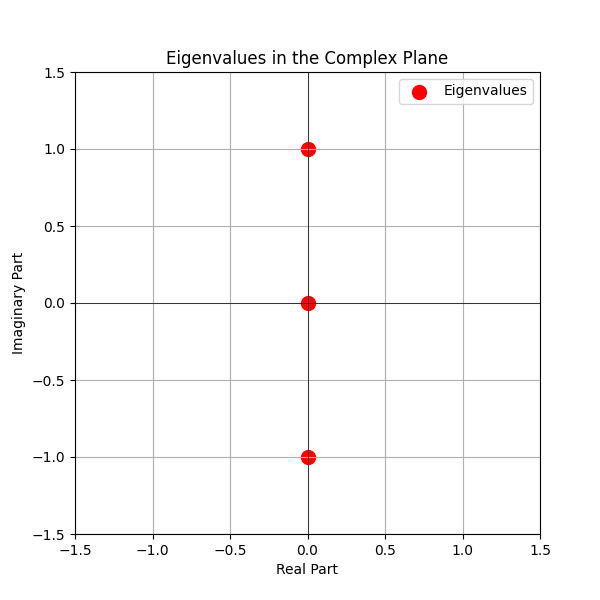
\includegraphics[width=0.85\columnwidth]{figs/graph-20.png}
    \caption{12.130}
    \label{fig:placeholder}
\end{figure}
\end{document}
